\section{Разработанное решение}
\label{sec:Chapter4} \index{Chapter4}
    \begin{figure}
        \centering
        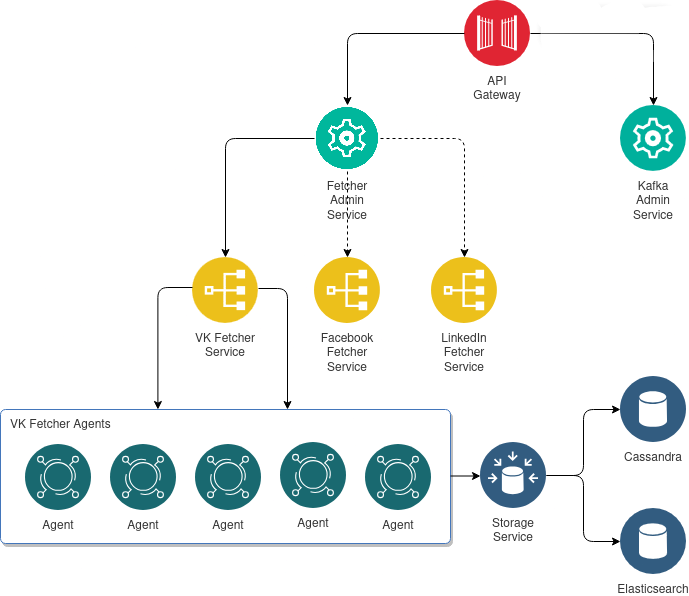
\includegraphics[scale=0.5]{architecture_diagram.png}
        \caption{Диаграма архитектуры}
    \end{figure}
    Как установлено в предыдущем разделе, проектируемая система требует одновременного обеспечения низкой задержки обработки, горизонтальной масштабируемости и устойчивости к сбоям. Реализация этих требований достигается через гибридную архитектуру, интегрирующую принципы Каппа-архитектуры с микросервисным подходом. Данный синтез формирует основу для обработки потоковых данных социальных сетей, обеспечивая баланс между производительностью, гибкостью и надёжностью.\\

    Все микросервисы системы можно отнести к нескольким слоям: \textbf{Cлой приёма данных}, \textbf{Cлой обработки}, \textbf{Cлой хранения и визуализации} и \textbf{Cлой управления и администрации}. Каждый микросервис связан с другими через топики Kafka.

    \subsection{Слой управления и администрации}
        Слой управления и администрации является главным управляющим уровнем системы. На данным слое находятся сервисы отвечающие за непосредственное управление системой.
        
        \subsubsection{Взаимодействие сервисов}
            Каждый сервис взаимодействует с другоми через Kafka. Для этого используется формат JSON. Каждая команда имеет следующую структуру:
            \begin{lstlisting}
                {
                    "target_type":
                    "content": {
                    }
                }
            \end{lstlisting}
            В поле \texttt{target\_type} устанавливает получатель тип команды, используя который, система определяет какую из структур команды использовать и обрабатывает содержимое поля \texttt{content} соответствующим образом.

            В рамках работы системы, для удобства обрыботки команд используется внутренняя структура данных, которая предварительно трансформируется в JSON и кодируется. Для создания команд используется внутренний класс-конструктор, а для трансформации - класс-обработчик. Эти классы изолированы и автоматически используются внутри специальзированной обёртка над Продюсером Kafka. Это позволяет снизить зависимости внутри системы и реализовывать взаимодействие системы без загромождения кода лишними вызовами обработчиков, что увеличивает читаемость кода и упрощает интеграцию в проект, а так же упрощает отладку. Для обратного декодирования из JSON во внутреннюю структуру используется библиотека \texttt{dacite}.

        \subsubsection{Kafka Admin Service}
            Kafka Admin Service — это сервис отвечающий за управление и администрирование Kafka. При инициализации он создаёт служебный топик и начинает обрабатывать приходящие в него команды. Основными ответственностями этого сервиса является создание и удаление топиков а так же их конфигурация, создание партиций. Через этот сервис проходит вся настройка работы Kafka.  

            Для взаимодействия с данных сервисом используется следующий формат \texttt{content}:
            \begin{lstlisting}
                "content": {
                    "command_type":
                    "id":
                    "topics_names": []
                    "topics_parameters": {
                        "name": []
                    }
                }
            \end{lstlisting}
            Где:
            \begin{itemize}
                \item \texttt{command\_type} — тип полученной команды, обозначающий целевое действие (создание топика, удаление) и влияющее на то, какие поля запроса будут использоваться.
                \item \texttt{id} — Уникальный идентификатор запроса.
                \item \texttt{topics\_names} — Список имён топиков.
                \item \texttt{topics\_parameters} — Список параметров топиков. Для каждого топика из списка имён сдесь должны быть приведены соответсвующие параметры, а именно колличество партиций и уровень реплицирования.
            \end{itemize}

        \subsubsection{Fetcher Admin Service}
            Fetcher Admin Service — это сервис отвечающие за администрацию сбора данных. Он не занимается сбором самостоятельно, а управляет сервисами по сборке данных из различных социальных сетей, например VK Fetcher Service. Основной обязанностью данного сервися является управление слоем приёма данных: добавление новых API токенов и удаление старых, управление списком обрабатываемых сообществ социальных сетей, добавление новых и удаление старых.

            Для взаимодействия с данных сервисом используется следующий формат \texttt{content}:
            \begin{lstlisting}
                "content": {
                    "command_type":
                    "id":
                    "social_media_type":
                    "groups": []
                    "APIToken":
                }   
            \end{lstlisting}
            Где:
            \begin{itemize}
                \item \texttt{command\_type} — тип полученной команды, обозначающий целевое действие (добавление API-токена, добавление сообществ в обработку) и влияющее на то, какие поля запроса будут использоваться.
                \item \texttt{id} — Уникальный идентификатор запроса.
                \item \texttt{social\_media\_type} — типо социальной сети, к которой отправляется запрос (VK, Twitter и тд)
                \item \texttt{groups} — Список групп / сообществ для добавления в обработку или удаления из неё.
                \item \texttt{APIToken} — Токен для добавления или удаления
            \end{itemize}

    \subsection{Слой приёма данных}
        Слой приёма данных — это слой системы, но котором расположены сервисы, отвечающие за сбор данных и отправку их для дальнейшей обработки в топики Kafka. На этом уровне так же реализуется обработка всех команд, с учётом особенностей системы. 

        \subsubsection{Особенности работы с VK}
            VK обладает открытым API, получить доступ к которому не составляет большого труда. Он предоставляет возможность для авторизации пользователя и собора открытой информации. Например такой информацией являются публикации в открытых группах, реакции на эти публикации и комментарии к ним. Так же с помощью Open API можно получить информацию о подписчиках сообществ, друзьях пользователей, фотографиях, видеозаписях и другой информацией, открытой пользователю. Иначе говоря VK API - это интерфейс, который позволяет получать информацию из базы данных vk.com с помощью HTTP-запросов к специальному серверу. Синтаксис запросов и тип возвращаемых ими данных строго определены на стороне самого сервиса. В ответ на запрос сервер возвращает ответ в формате JSON, что стоит учесть при выборе технологий, используемых для проектирования системы. \\

            Для отправки API-запросов используется  формат HTTP, в частности методы POST или GET. В API VK эти методы равнозначны. Запросы отправляются на адреса следующего вида:

            \texttt{https://<адрес>/method/<API-метод>?<параметры>} \\

            Где:    
            \begin{itemize}
                \item \texttt{<адрес>} — один из адресов API ВКонтакте:
                \begin{itemize}
                    \item \texttt{api.vk.com}
                    \item \texttt{api.vk.ru}
                \end{itemize}
                \item \texttt{<API-метод>} — имя раздела и API-операции для вызова, например \texttt{users.get} или \texttt{likes.add}
                \item \texttt{<параметры>} — параметры, которые передаются методу в строке запроса, например \texttt{...?v=5.199\&p1=v1}. Так же их называют query-параметрами.
            \end{itemize}

            VK API, как и API других социальных сетей, имеет ряд ограничений, которые стоит учитывать при проектировании системы:
            \begin{enumerate}
                \item Максимум 3 запроса / секунду с одного API-ключа.
                \item Для \texttt{wall.get} возвращается $\leq$ 100 последних постов в сообществе.
                \item Невозможность подписки на события в реальном времени.
                \item Невозможность получения удалённых/скрытых постов.
            \end{enumerate}

        \subsubsection{VK Fetcher Service и VK Fetchers}
            VK Fetcher Service является центральным сервисом сбора данных социальной сети VK и управляется из Fetcher Admin Service. При инициализации он отправляет запрос в Kafka Admin Service на создание служебного топика для приёма команд от Слоя управления и администрации.

            Для каждого из API-токенов VK Fetcher Service создаёт отдельный инстанс Фетчера, который в асинхронном порядке обрабатывает группы сообществ в обработке. Это нужно для того, что бы обойти ограничение на частоту запросов к API.

            После инициализации сервиса, тот разделяется на 2 асинхронных потока, один из которых обрабатывает приходящие из Слоя управления команды, а второй создаёт очередь задач. Он начинает создавать задачи на обновление данных по конкретной группе из списка сообществ на обработку, после чего складывает их в очередь. Каждый из Фетчеров в свою очередь читает эти задачи и создаёт асинхронную задачу для разпараллеливания нагрузки, после чего уходит в ожидание на $0.5$ секунды для соблюдения правил работы с API. Подобная архитектура позволяет уменьшить время простоев, одновременно регулируя и балансируя нагрузку на разные API-токены. Ещё одним приемуществом подобной архитектуры является возмжность динамически регулировать список обрабатываемых групп, а так же добавлять новые ключи, не останавливая работу сервису. Это крайне важно для регулирования больших всплесков активности и поддержания масштабируемости.

    \subsection{Слой обработки}
        Слой обработки выступает как главный рабочий слой. Он отвечает за предварительную обработку данных, их агрегацию и соверщение перобразований над ними (добавление данных, удаление ненужных и тд). Для этого используется пайплайн Kafka + Flink:             

        \subsubsection{Интеграция с Kafka}
            Kafka выступает в роли шины событий, обеспечивая надежную передачу данных между микросервисами. Сообщения группируются по топикам в зависимости от типа данных (например, посты, комментарии, внутренние команды). Для соблюдения упорядоченности данных ключи сообщений вычисляются на основе идентификатора группы, гарантируя последовательную обработку постов. 
            
            Внутри системы реализована специальная обёртка над Продюсером, которая инкапсулирует в себе предварительную обработку данных перед отправкой в топик (например преобразование в JSON). Так же перед отправкой данные кодируются в UTF-8 для обработки рускоязычного текста.
            
        \subsubsection{Интеграция с Flink}
            Apache Flink занимает центральное место в архитектуре системы, выступая в качестве высокопроизводительного движка потоковой обработки, который обеспечивает преобразование, агрегацию и анализ данных в режиме реального времени. Его интеграция в систему основана на принципах Каппа-архитектуры, что позволяет обрабатывать как текущие события, так и исторические данные через единый вычислительный конвейер, устраняя необходимость в раздельных системах для потоковой и пакетной обработки.

            Flink выполняет критически важную функцию моста между источником данных (Apache Kafka) и системами хранения/аналитики (Elasticsearch и Cassandra). Основная задача Flink в системе — обеспечить обработку каждого поста из социальной сети VK с задержкой менее 60 секунд от момента публикации до сохранения результатов. Это достигается за счет непрерывной обработки событий, преобразований данных в реальном времени и управления состоянием вычислений при длительных операций. 

            Источником данных для Flink выступают топики Apache Kafka, куда VK Fetcher Service отправляет сырые данные из социальной сети. Flink потребляет эти данные через распределенного потребителя. Ключевой особенностью является использование механизма водяных знаков (watermarks), которые позволяют Flink определять полноту данных в потоке и корректно обрабатывать события, приходящие с задержкой из-за особенностей сети или неравномерной нагрузки в социальной сети.

            Проходящие через Flink данные проходят следующие этапы преобразований:
            \begin{enumerate}
                \item \textbf{Нормализация и очистка} \\
                В первую очередь это приведение временных меток к единому формату ISO 8601, фильтрация некорректных или повреждённых записей, а так же стандартизация текстовых данных (приведение к одному регистру, нормальзация кодировки)
                \item \textbf{богащение контекстом} \\
                На этом этапе добавляются дополнительные данные. Это добавление извлечение методанных, классификация тональности с помощью ML-моделей или любые дополнительные данные, которые могут помочь на следующем этапе.
                \item \textbf{Оконная агрегация} \\
                На этом этапе выполняется расчет скользящих средних показателей (лайки, репосты) в 5-минутных окнах и обнаружение аномалий активности через статистические методы. Данный этап являтся главным для потоковой обработки.
            \end{enumerate}

            Для управления задачами в кластере Flink используется job-manager-ui, доступ к котрому пробрасывается из кластера Flink

    \subsection{Слой хранения и визуализации}
        Данный слой не реализовывался в прототипе, однако стоит отдельно упомянуть. На данном слое располагаются сервисы ответственные за хранение и подготовку данных к глубокому анализу и пакетной обработке.

        \subsubsection{Storage Service}
            Storage Service служит основным сервисом сохранения данных. Он читает полученные от Фетчеров данные, после чего сохраняет их в 2 хранилища: \textbf{Elasticsearch} (горячее хранилище) для быстрого поиска и дополнительной аналитики и \textbf{Cassandra} (холодное хранилище) для долгосрочного хранения и интеграции с глубокой, пакетной обработкой данных за большие промежутки времени. 

        \subsubsection{Elasticsearch}
            Elasticsearch интегрирован в систему как ключевой компонент для оперативной аналитики, обеспечивающий полнотекстовый поиск, агрегацию данных и визуализацию в режиме реального времени. В архитектуре системы он выполняет роль горячего хранилища и основного движка аналитики. Опционально Elasticsearch так же можно использовать для визуализации через интеграцию с Kibana. Индексы настроены с анализаторами для русскоязычного контента. Агрегации по временным гистограммам позволяют визуализировать активность пользователей. Для сохранения данных в Elasticsearch используется официальный коннектор Flink \texttt{org.apache.flink.connector\\.elasticsearch7}

            Данные поступают из Apache Flink через REST API с использованием bulk-запросов для оптимизации производительности. Для поддержания уникальности используется состовной ключ \texttt{group\_id\_post\_id}, который гарантирует уникальность записей.

        \subsubsection{Cassandra}
            CApache Cassandra в системе выполняет роль высокомасштабируемоего распределенного хранилища для долгосрочного хранения больших объемов данных. В архитектуре системы она выполняет функции основного хранилища для сырых данных и агрегированных показателей, платформы для исторического анализа данных за длительные периоды и системы резервного копирования. Схема таблиц может быть оптимизирована для высокой скорости записи, а горизонтальная масштабируемость достигнута без изменения архитектуры добавлением новых нод.  

            Ключевое пространство social\_media может быть организовано с учетом специфики социальных данных. Это достигается за счёт стратегии репликации: NetworkTopology-Strategy обеспечивает копирование данных между дата-центрами (например, 3 копии в основном DC, 2 - в резервном), а так же проектированием таблиц с опорой на особенности данных. Основные таблицы:
            \begin{itemize}
                \item \textbf{raw\_posts} — Хранит исходные данные постов с партиционированием по ID группы
                \item \textbf{daily\_aggregates} — Содержит предварительно агрегированные дневные метрики (количество постов, средние лайки/комментарии)
                \item \textbf{backups} — Архивные копии данных из Elasticsearch
            \end{itemize}

            Для повышения безопасности и отказоустойчивости, данные раз в несколько дней копируются из Elasticsearch и распределяются по дата-центрам, каждая копия содержит метку времени и идентификатор источника.

    \subsection{K8S}
        Для упрощения запуска системы, её развёртывания и масштабирования, для каждого сервиса был написан Dockerfile и yml-файл, что позволяет запустить систему в K8S. Это значительно упрощает управление системой, открывает доступ к реализации автоматического масштабирования любого сервиса и оркестризации. Так же это упрощает интеграцию с Flink и Kafka, за счёт использования уже готовых Docker-образов. 
    
    \subsection{Соответствие требованиям}
        Соответствие требованиям подтверждено замерами задержки в обработке сообществ ВК. Замерялось время обработки всех сообществ из списка обработки.  Для удобства анализа данные изображены на графике. 
        \begin{figure}
            \centering
            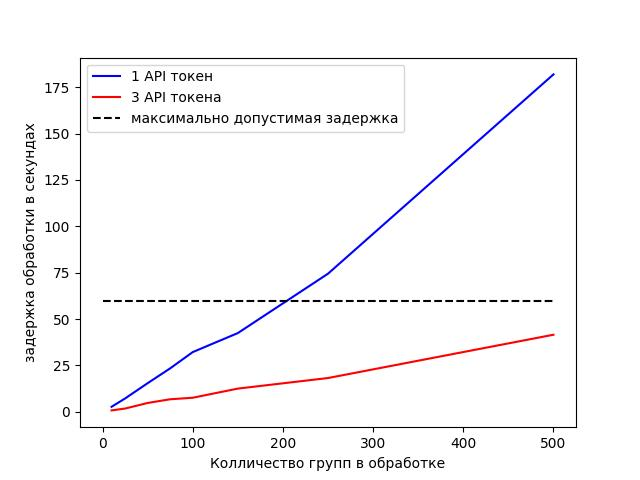
\includegraphics[scale=0.7]{benchmark.jpeg}
            \caption{График задержки обработки}
        \end{figure}

        Как можно заметить главным узким местом системы, как и предполагалось является отправка и обработка запросов VK. Однако при масштабировании колличества API-токенов, система автоматически использует новые ресурсы и задержка значительно снижается. Таким образом для обработки 500 групп достаточно 3-х API-токенов, а для обработки 10000 сообществ с задержкой менее минуты, достаточно 50 токенов.

        Так же были сняты замеры времени обработки одного сообщества. Для прохождения всего пайплайна сообществом, системе необхадимо $0.4$ секунды.
        
    \subsection{Исследование системы на предмет улучшений и ускорения}
        Для разработанной системы был проведён анализ узких мест и предложены варианты для их улучшения и оптимизации:
        \begin{enumerate}
            \item Одним из самых узких мест в системе оказалась ситема фетчинга данных социальных сетей. Для решения этой предлагаются следующие улучшения: автоматическое удаление недоступных и закрытых сообществ, оптимизация обновления данных группы, основываясь на частоте публикаций в сообществе. Нарпимер сообщество которое публикует новости раз в сутки менее целесообразно опрашивать каждую минуту, в отличии от сообществ, публикующих данные каждые 10 минут. Динамически настраивая подобные параметры, можно добиться ускорения в несколько раз. Однако всё ещё нужно оставить возможность отключения этой функции для конкретных сообществ, для сообществ, требующих максимально высокой точности и низкой задержки.
            \item Ускорение Flink-Обработки возможно достичь с помощью предварительной агрегации данных и оптимизации состояний, а так же векторизации обработки. таким образом можно будет достичь сокращение времени обработки окон на $25-35\%$ 
            \item Оптимизация Доступа к Данным может стать необхадима при увеличении колличества обрабатываемых данных. Для Elasticsearch этих оптимизаций можно достичь за счёт гибридного кэша в Radis (самые активыне сообщества и пользователи) и прекомпиляции шаблонов запросов.
            \item В случае необхадимости оптимизации Kafka, например при росте задержек при малом размере сообщений, можно воспользоваться сжатием данных, перед отправкой в Kafka, например при помощи настройки Kafka (compression\_type="snappy") или использованием zstd
        \end{enumerate}
        
\newpage
